\documentclass{article}

\usepackage[main=english,vietnamese]{babel}
\usepackage[T1]{fontenc}
\usepackage[utf8]{inputenc}
\usepackage[sexy]{evan}
\usepackage{matchsticks}
\usepackage{wrapfig}
\usepackage{listings}

\newtheorem{hint}{Hint}

\title{Pigeonhole Principle in Combinatorial Geometry}
\author{Nghia Doan}
\date{\today}

\begin{document}

\maketitle

In this article, we show two examples that can be solved with the Pigeonhole Principle.

\begin{definition*}[Pigeonhole Principle]
    \label{definition:pigeonhole-principle}
    The Pigeonhole Principle (also known as the Dirichlet box principle, Dirichlet principle or box principle)
    states that if $n + 1$ or more holes are placed in $n$ pigeons, then one pigeon must contain two or more holes.
    Another definition could be phrased as among any $n$ integers, there are two with the same modulo-$n-1$ residue.

    The extended version of the Pigeonhole Principle states that if $k$ objects are placed in $n$ boxes
    then at least one box must hold at least $\left\lceil \frac{k}{n} \right\rceil$ objects.
    Here $\lceil \cdot \rceil$ denotes the ceiling function.
\end{definition*}

\begin{example*}[One]
    \label{example:one}
    There are $101$ points in a unit square.
    Prove that five of them can be covered by a circle radius $\frac{1}{7}.$ 
\end{example*}

\begin{remark*}
    \textit{The idea: the idea comes from the given number of points $101$ is just one more than $4 \times 25,$
    which means that if we divide the square into $25$ \textit{holes},
    then among $101$ points, or \textit{pigeons}, there are $5$ of them should be in a \textit{hole.}
    The easiest way to divide a square into $25$ pieces is to divide it into $5 \times 5$ grid.}
\end{remark*}

\begin{proof}[\nameref{example:one}]
    Lets divide the unit square into $5 \times 5 = 25$ squares as shown below.
    \begin{figure}[h]
        \centering
        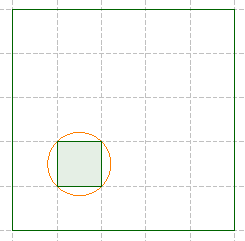
\includegraphics[width=3.5cm]{./svg/pdf/2022-2-ms-1-2.pdf}
    \end{figure}

    According to the Piegonhole Principle,
    there exists a square where at least $\left \lceil \frac{101}{25} \right \rceil = 5$ points reside.
    The circle centered at the center of the square radius $\frac{1}{7}$ cover the whole square since,
    \[ 
        \text{half of the diagonal of the square,\ }\frac{1}{2} \cdot \frac{\sqrt{2}}{5}  < \boxed{\frac{1}{7}.}
    \]
\end{proof}

\newpage
    
\begin{example*}[Two]
    \label{example:two}
    For $\textbf{n} \ge 1,$ on a $2n \times 2n$ board, $3n$ squares are marked.
    Prove that $n$ rows and $n$ columns can be selected so that they contain all marked squares.
\end{example*}

\begin{remark*}
    First, we \textit{get our hand dirty} by drawing some examples and see how it works.
    In the example below, where $n=4$, in a $8\times 8$ board we choose rows $2,5,7$ and $8;$ then columns $d,f,g$ and $h$
    to cover all marked squares.
    Note that rows $2,5,7,$ and $8$ cover $8 = 2 \times 4$ marked squares.

    \textit{Is it possible that $n$ rows can be chosen such that they cover some $2n$ marked squares?}

    How about trying to select $n$ rows so that they cover as many unmarked squares as possible?
    
    This is called a \textit{greedy} approach. A \textbf{greedy algorithm} is an algorithm
    that follows the problem-solving heuristic of making the locally optimal choice at some stage.
    A greedy strategy might not produce an optimal solution, but it can help to find a solution.
\end{remark*}

\begin{table}[h]
    \centering
    \begin{tabular}{ccccccccc}
                        & a                      & b                                             & c                                             & d                                             & e                                             & f                                             & g                                             & h                                             \\ \cline{2-9} 
    \multicolumn{1}{c|}{8} & \multicolumn{1}{c|}{x} & \multicolumn{1}{c|}{{\color[HTML]{FFFFFF} x}} & \multicolumn{1}{c|}{{\color[HTML]{FFFFFF} x}} & \multicolumn{1}{c|}{{\color[HTML]{FFFFFF} x}} & \multicolumn{1}{c|}{{\color[HTML]{FFFFFF} x}} & \multicolumn{1}{c|}{{\color[HTML]{FFFFFF} x}} & \multicolumn{1}{c|}{{\color[HTML]{FFFFFF} x}} & \multicolumn{1}{c|}{{\color[HTML]{FFFFFF} x}} \\ \cline{2-9} 
    \multicolumn{1}{c|}{7} & \multicolumn{1}{c|}{}  & \multicolumn{1}{c|}{x}                        & \multicolumn{1}{c|}{}                         & \multicolumn{1}{c|}{}                         & \multicolumn{1}{c|}{}                         & \multicolumn{1}{c|}{}                         & \multicolumn{1}{c|}{}                         & \multicolumn{1}{c|}{x}                        \\ \cline{2-9} 
    \multicolumn{1}{c|}{6} & \multicolumn{1}{c|}{}  & \multicolumn{1}{c|}{}                         & \multicolumn{1}{c|}{}                         & \multicolumn{1}{c|}{}                         & \multicolumn{1}{c|}{}                         & \multicolumn{1}{c|}{}                         & \multicolumn{1}{c|}{x}                        & \multicolumn{1}{c|}{}                         \\ \cline{2-9} 
    \multicolumn{1}{c|}{5} & \multicolumn{1}{c|}{}  & \multicolumn{1}{c|}{}                         & \multicolumn{1}{c|}{x}                        & \multicolumn{1}{c|}{}                         & \multicolumn{1}{c|}{x}                        & \multicolumn{1}{c|}{}                         & \multicolumn{1}{c|}{}                         & \multicolumn{1}{c|}{}                         \\ \cline{2-9} 
    \multicolumn{1}{c|}{4} & \multicolumn{1}{c|}{}  & \multicolumn{1}{c|}{}                         & \multicolumn{1}{c|}{}                         & \multicolumn{1}{c|}{}                         & \multicolumn{1}{c|}{}                         & \multicolumn{1}{c|}{x}                        & \multicolumn{1}{c|}{}                         & \multicolumn{1}{c|}{}                         \\ \cline{2-9} 
    \multicolumn{1}{c|}{3} & \multicolumn{1}{c|}{}  & \multicolumn{1}{c|}{}                         & \multicolumn{1}{c|}{}                         & \multicolumn{1}{c|}{x}                        & \multicolumn{1}{c|}{}                         & \multicolumn{1}{c|}{}                         & \multicolumn{1}{c|}{}                         & \multicolumn{1}{c|}{}                         \\ \cline{2-9} 
    \multicolumn{1}{c|}{2} & \multicolumn{1}{c|}{}  & \multicolumn{1}{c|}{}                         & \multicolumn{1}{c|}{x}                        & \multicolumn{1}{c|}{x}                        & \multicolumn{1}{c|}{}                         & \multicolumn{1}{c|}{x}                        & \multicolumn{1}{c|}{}                         & \multicolumn{1}{c|}{}                         \\ \cline{2-9} 
    \multicolumn{1}{c|}{1} & \multicolumn{1}{c|}{}  & \multicolumn{1}{c|}{}                         & \multicolumn{1}{c|}{}                         & \multicolumn{1}{c|}{}                         & \multicolumn{1}{c|}{}                         & \multicolumn{1}{c|}{}                         & \multicolumn{1}{c|}{}                         & \multicolumn{1}{c|}{x}                        \\ \cline{2-9} 
    \end{tabular}
\end{table}     

\begin{proof}[\nameref{example:two}]
    We first prove the claim we have noted in the remark.
    
    \begin{claim*}
        Lets choose $n$ rows such that \textbf{each of them cover as many squares as possible.}
        Then these rows cover at least $2n$ marked squares.
    \end{claim*}
    
    \begin{subproof}
        Assume that the number of marked squares covered by these square is less than $2n,$
        then there are more than $3n-2n=n$ squares \textit{not covered} by them,
        therefore the \textit{non-selected} $n$ rows cover at least $n+1$ squares.

        According to the Piegonhole Principle, there is one \textit{non-selected} row
        that contains at least two marked squares.
        But by choice as above, \textbf{each of the selected rows should have at least as many markered squares
        as a non-selected rows,} thus the selected ones should cover at least $2n$ squares.

        Then the number of marked squares covered by all square is at least $2n+(n+1) = 3n+1.$
        This exceeds the number of marked squares, which is $3n,$ thus it is impossible.
    \end{subproof}

    Hence, at least $2n$ marked squares are covered by \framebox{$n$ selected rows.}
    For at most $n$ remaining uncovered squares, it is easy to choose \framebox{$n$ columns.}
\end{proof}

\end{document}